\documentclass[12pt, a4paper]{report}
\usepackage[russian]{babel}
\usepackage{geometry}
\usepackage{graphicx}


\newgeometry{
	left=2cm,
	right=2cm
}

\author{Босенко Борис Игоревич}
\title{Численные методы вычисления интегралов.\\ Индивидуальная часть.}

\pagestyle{empty}

\begin{document}
	
	\maketitle
	
	\tableofcontents
	
	\pagestyle{plain}
	
	\addcontentsline{toc}{chapter}{Задание}
	\section*{Задание}
	
	\begin{enumerate}
	
		\item Составить интегральную сумму для интеграла Римана функции $f(x) = x^2$ по промежутку $[1, 2]$.
		\item Вычислить интеграл через предел интегральных сумм. 
		\item Доказать, что соответствующий интеграл существует. 
		\item Проверить вычисление при помощи формулы Ньютона-Лейбница. 
		\item Написать программу, вычисляющую и отрисовывающую интегральные суммы для данной функции на данном отрезке. Входные данные для программы: число точек разбиения, способ выбора оснащения (левые, правые, средние, трапеция). 
		\item Найти погрешность оценки, сравнить её с теоретической погрешностью. 
		\item Вывести формулы для оценки погрешности. 
	
	\end{enumerate}

	\newpage
	
	
	\addcontentsline{toc}{chapter}{Аналитическая часть}
	\section*{Аналитическая часть}
	
	\
	
	Для данной функции предел интегральных сумм Римана будет выглядеть как 
	\[I = \lim_{\Delta x \to 0} \sum_{k=1}^{n} f(\xi_k)\Delta x \]
	
	Так как разбиение равномерное, для числа разбиений n можем посчитать координаты точек разбиения по формуле
	
	\[x_k = 1 + \frac{k}{n} ( 2 - 1 ) = 1 + \frac{k}{n}, k \in \{0, ..., n\}\]
	
	Тогда можем посчитать данный интеграл с помощью формулы правых прямоугольников
	
	\[ I = \lim_{\Delta x \to 0} \sum_{k=1}^{n} f(\xi_k)\Delta x = \lim_{\frac{1}{n} \to 0} \sum_{k=1}^{n} \left( f\left(1 + \frac{k}{n}\right) \frac{1}{n} \right) = \lim_{n \to \infty} \left( \frac{1}{n} \sum_{k=1}^{n} \left( 1 + \frac{k}{n}\right)^2 \right)  = \]
	\[ = \lim_{n \to \infty} \left( \frac{1}{n} \sum_{k=1}^{n} \left( 1 + 2\frac{k}{n} + \frac{k^2}{n^2} \right)  \right)  = \lim_{n \to \infty} \left( \frac{1}{n} \left( n + \frac{n(n+1)}{n} + \frac{n(n+1)(2n+1)}{6n^2} \right)  \right)  = \] 
	\[ = \lim_{n \to \infty} \left( 1 + \frac{n+1}{n} + \frac{(n+1)(2n+1)}{6n^2} \right)  = 1 + \lim_{n \to \infty} \frac{n+1}{n} + \lim_{n \to \infty} \frac{2n^2 + 3n + 1}{6n^2} = \]
	\[ = 1 + 1 + \frac{1}{3} = 2\frac{1}{3} = \frac{7}{3}\]
	
	При этом функция $f(x) = x^2$ интегрируема на промежутке $[1, 2]$, так как она непрерывна (и это является достаточным условием для существования интеграла.)
	
	Для сравнения, найдем значение этого интеграла по формуле Ньютона-Лейбница:
	
	\[ \int_{1}^{2} f(x) dx = \int_{1}^{2} x^2 dx = \frac{x^3}{3} \ \bigg|_{1}^{2} = \frac{8}{3} - \frac{1}{3} = \frac{7}{3}\]
	
	Таким образом, оба способа дали одинаковый результат.
	
	\newpage
	
	\addcontentsline{toc}{chapter}{Результаты работы программы}
	\section*{Результаты работы программы}
	
	\begin{center}
		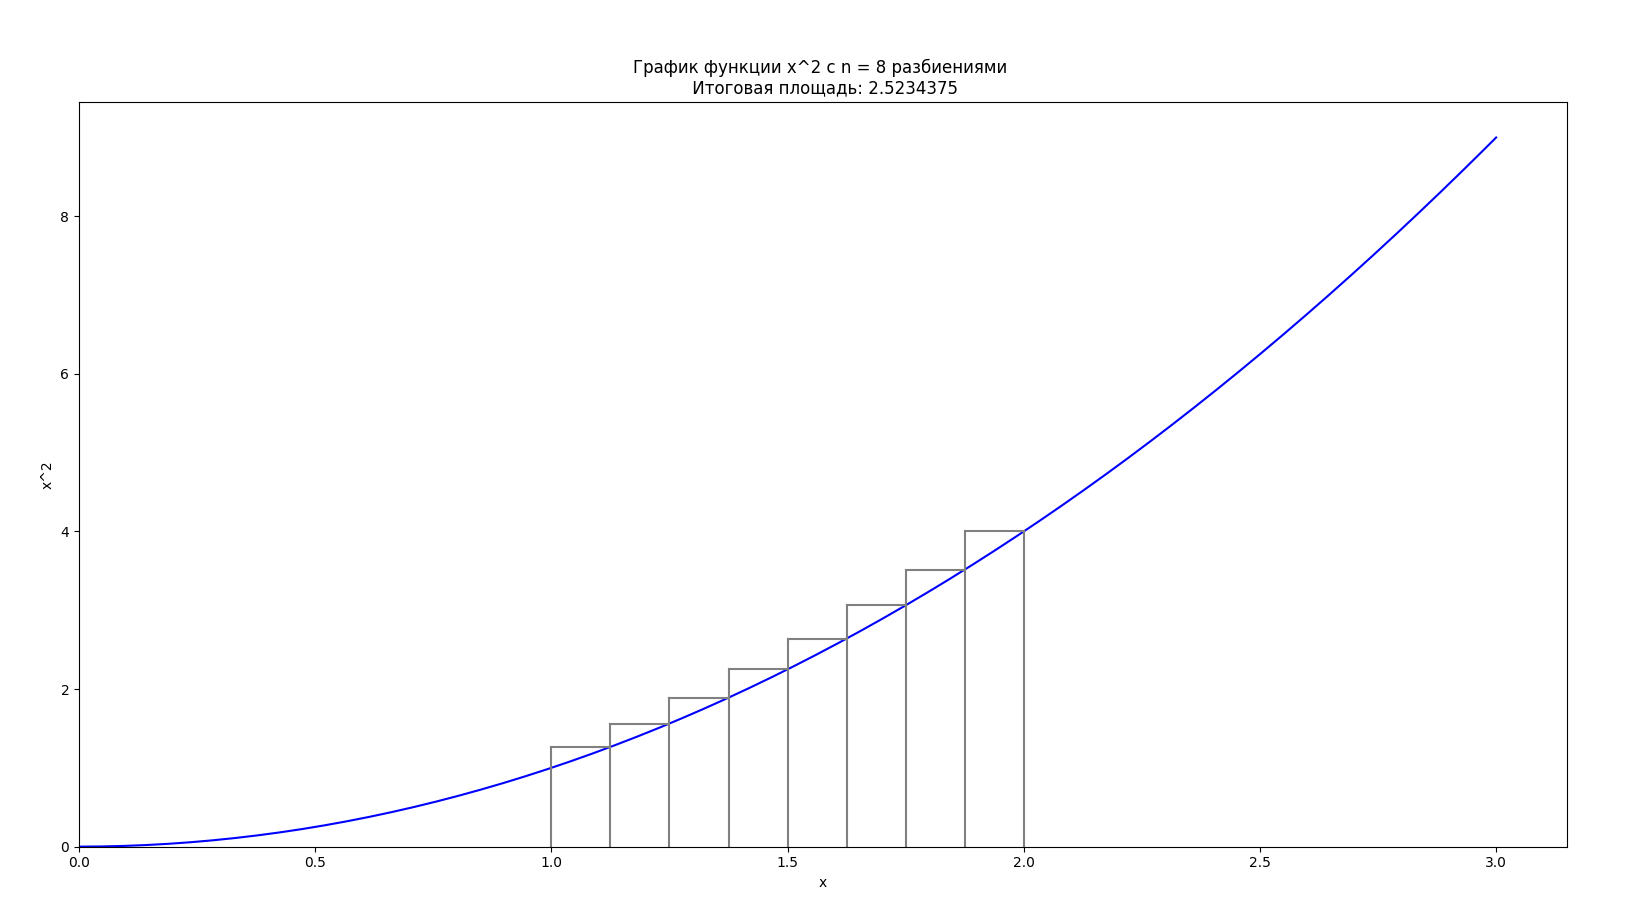
\includegraphics[scale=0.4]{Правые прямоугольники.png}
		Рисунок 1
		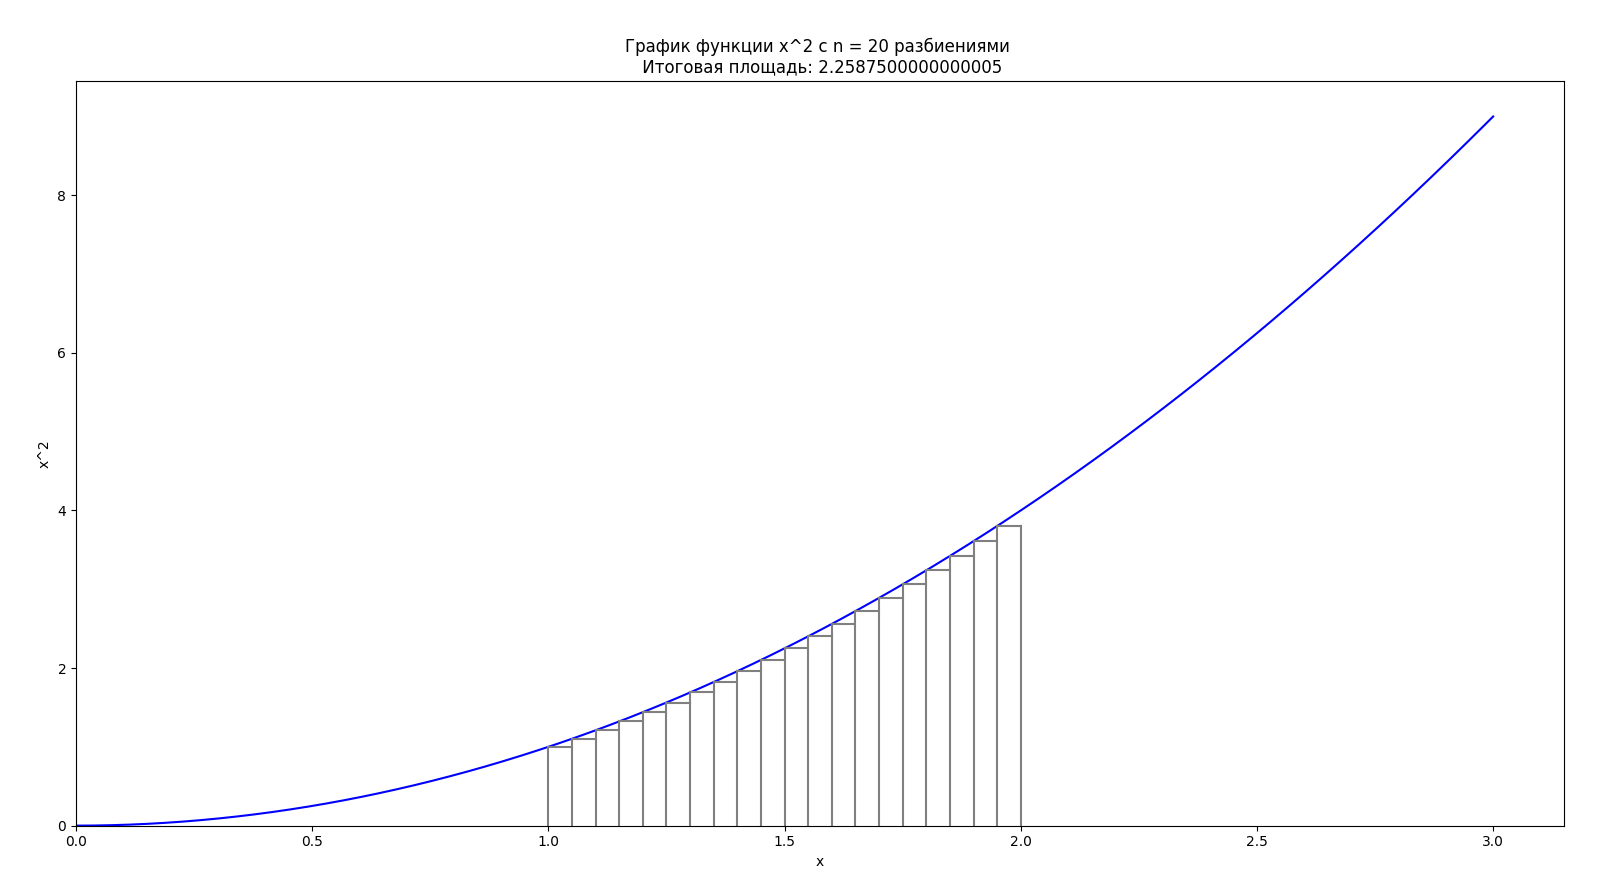
\includegraphics[scale=0.4]{Левые прямоугольники.png}
		Рисунок 2
		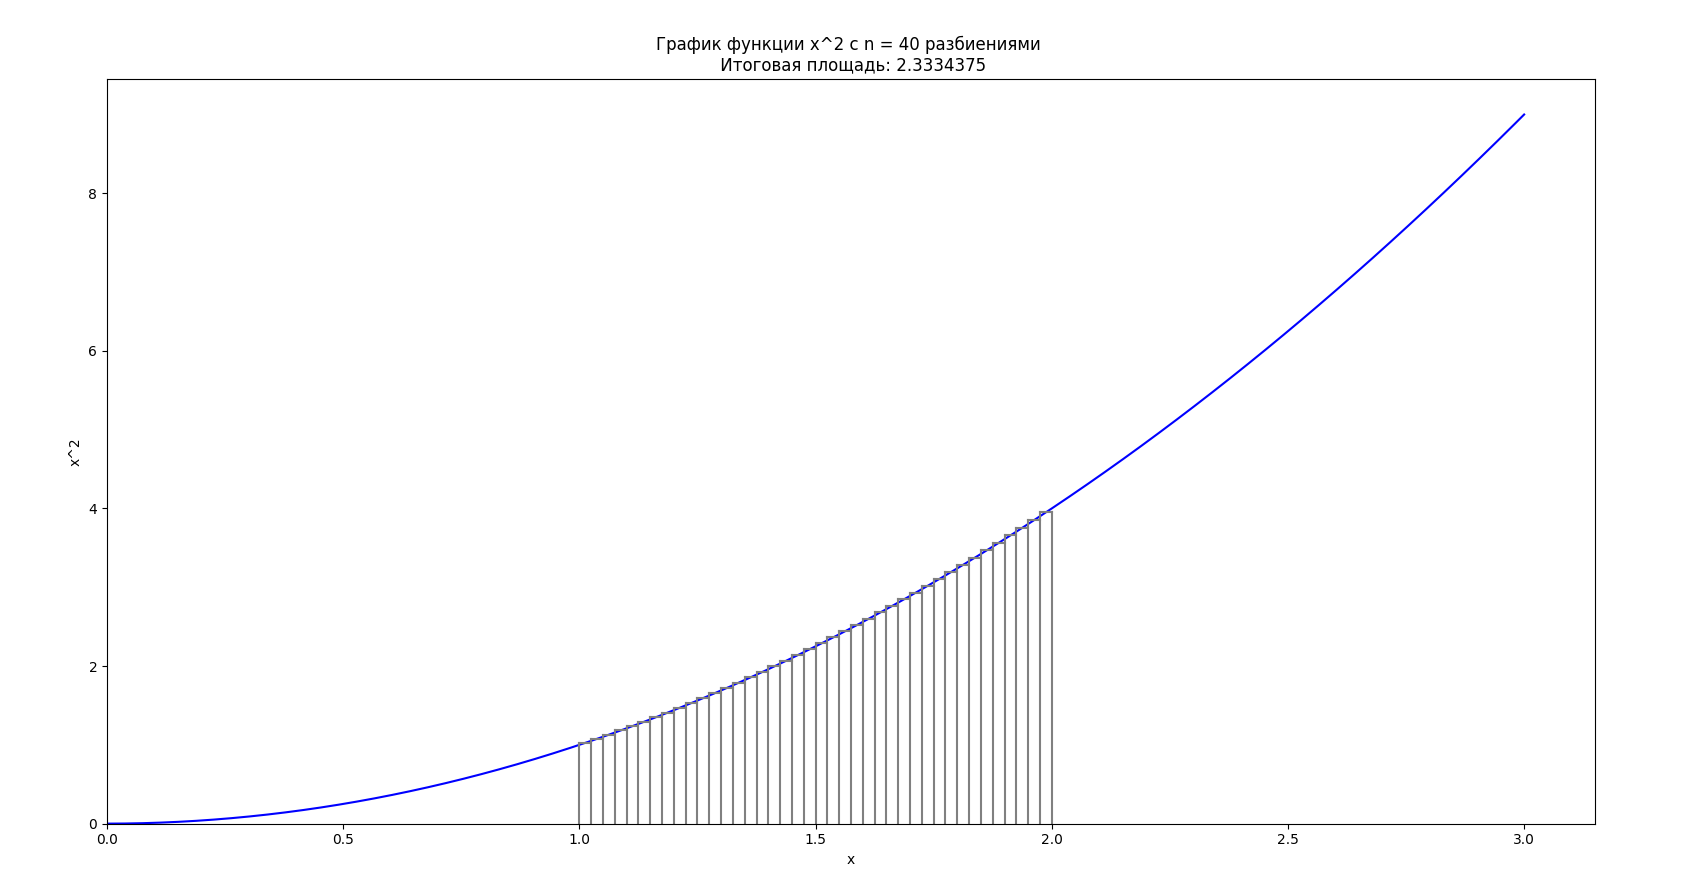
\includegraphics[scale=0.4]{Средние прямоугольники.png}
		Рисунок 3
		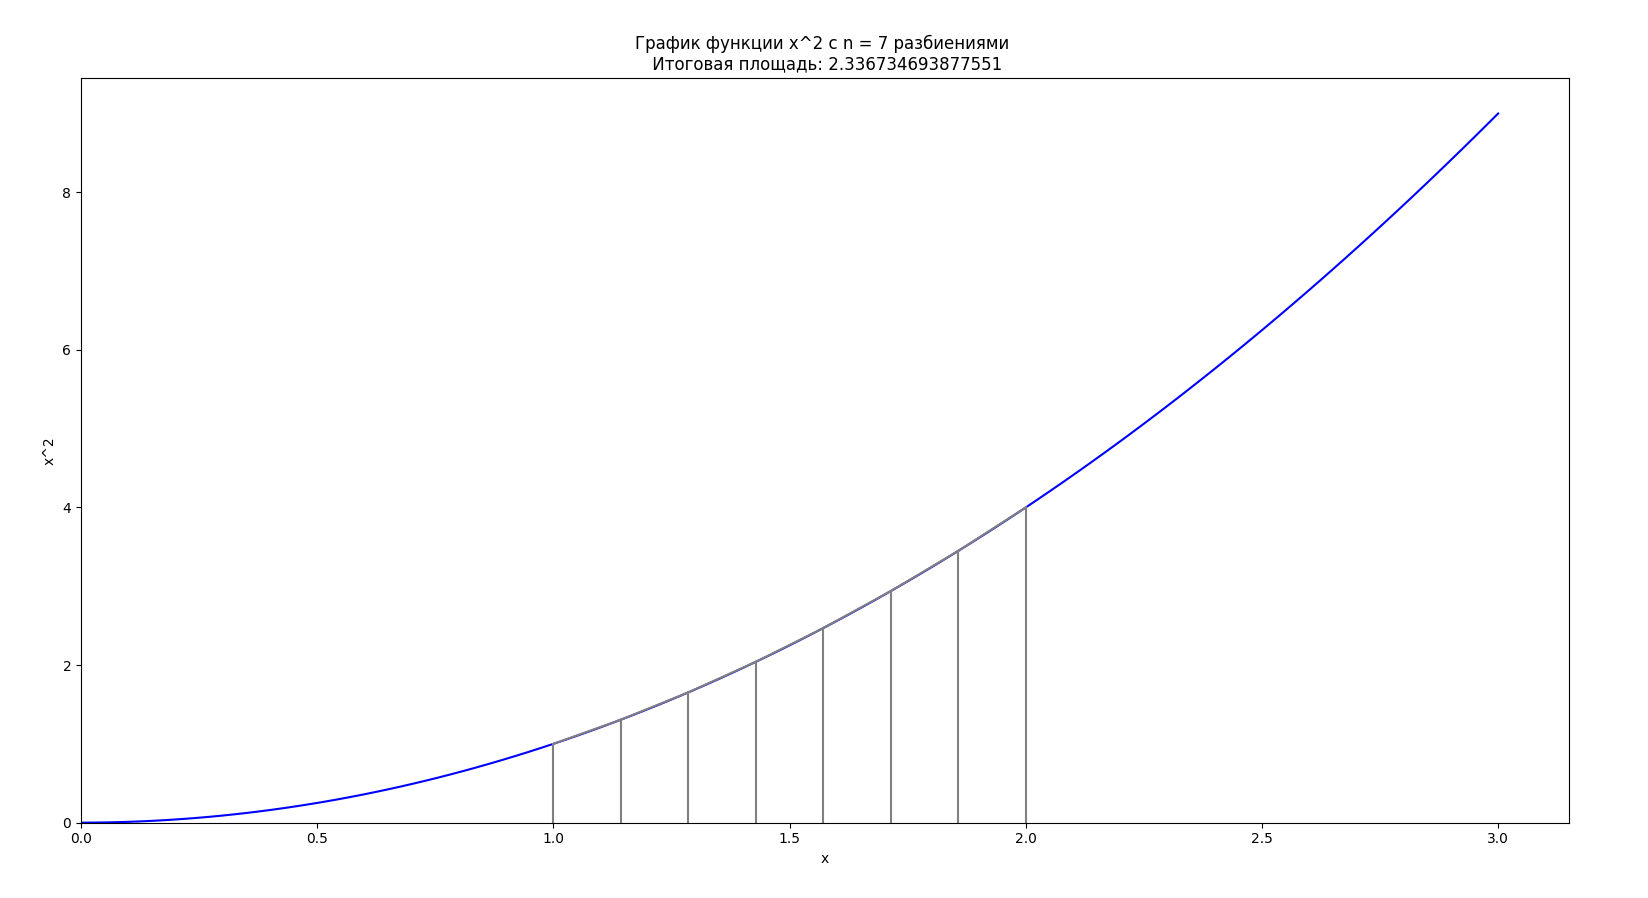
\includegraphics[scale=0.4]{Трапеции.png}
		Рисунок 4
	\end{center}
	
	\newpage
	
	\addcontentsline{toc}{chapter}{Вывод формул для погрешностей}
	\section*{Вывод формул для погрешностей}
	
	\textbf{Формула левых прямоугольников}
	
	Пусть $f \in C^1[a,b]$ \\ 
	Докажем формулу погрешности для левых прямоугольников. Для этого разложим функцию в ряд Тейлора с остатком в форме Лагранжа на промежутке $[x_{i-1}, x_i]$
	
	\[ f(x) = f(x_{i-1}) + f'(\xi)(x - x_{i-1}), \ \xi \in (x_{i-1}, x)\]
	
	Далее проинтегрируем обе части по отрезку $[x_{i-1}, x_i]$
	
	\[ \int\limits_{x{i-1}}^{x_i} f(x)dx = \int\limits_{x_{i-1}}^{x_i} f(x_{i-1})dx + \int\limits_{x_{i-1}}^{x_i} f'(\xi)(x - x_{i-1})dx\]
	
	Первый интеграл в правой части можно заменить на $f(x_{i-1}) \Delta x_i$, так как он равен площади одного прямоугольника, а значит выражение принимает вид 
	
	\[ \int\limits_{x{i-1}}^{x_i} f(x)dx = f(x_{i-1}) \Delta x_i + \int\limits_{x_{i-1}}^{x_i} f'(\xi)(x - x_{i-1})dx\]
	
	Далее перенесем это слагаемое влево и используем оценку $f'(\xi) \leq \max_{\Delta_i} |f'(x)|$, таким образом получив
	
	\[ \left| \int\limits_{x{i-1}}^{x_i} f(x)dx - f(x_{i-1}) \Delta x_i \right| \leq \max_{\Delta_i} |f'(x)| \int\limits_{x_{i-1}}^{x_i} (x - x_{i-1})dx\]
	
	Упростим левое выражение, избавившись от интеграла
	
	\[ \max_{\Delta_i} |f'(x)| \int\limits_{x_{i-1}}^{x_i} (x - x_{i-1})dx = \max_{\Delta_i} |f'(x)| \int\limits_{x_{i-1}}^{x_i} (x - x_{i-1})d(x - x_{i-1}) = \]
	\[ = \max_{\Delta_i} |f'(x)| \frac{(x-x_{i-1})^2}{2} \Bigg|_{x_{i-1}}^{x_i} = \frac{1}{2} \max_{\Delta_i} |f'(x)| (x_i - x_{i-1})^2 \]
	
	Если $ \Delta x_i = \frac{b-a}{n}$, то, просуммировав по всем n отрезкам, получим
	
	\[ \left| \int\limits_{a}^{b} f(x)dx - \sum_{i=1}^{n} f(x_{i-1}) \Delta x_i \right| \leq \frac{(b-a)^2}{2n^2} \sum_{i=1}^{n} \max_{\Delta_i}|f'(x)| \leq \frac{(b-a)^2}{2n} \max_{[a, b]}|f'(x)|\]
	
	Таким образом, формула доказана.
	
	\newpage
	
	\textbf{Формула правых прямоугольников}
	
	Практически аналогично доказывается формула правых прямоугольников.
	
	Пусть $f \in C^1[a,b]$ \\ 
	Разложим функцию в ряд Тейлора с остатком в форме Лагранжа на промежутке $[x_{i-1}, x_i]$
	
	\[ f(x) = f(x_i) + f'(\xi)(x - x_i), \ \xi \in (x, x_i)\]
	
	Далее проинтегрируем обе части по отрезку $[x_{i-1}, x_i]$
	
	\[ \int\limits_{x{i-1}}^{x_i} f(x)dx = \int\limits_{x_{i-1}}^{x_i} f(x_i)dx + \int\limits_{x_{i-1}}^{x_i} f'(\xi)(x - x_i)dx\]
	
	Первый интеграл в правой части можно заменить на $f(x_i) \Delta x_i$, так как он равен площади одного прямоугольника, а значит выражение принимает вид 
	
	\[ \int\limits_{x{i-1}}^{x_i} f(x)dx = f(x_i) \Delta x_i + \int\limits_{x_{i-1}}^{x_i} f'(\xi)(x - x_i)dx\]
	
	Далее перенесем это слагаемое влево и используем оценку $f'(\xi) \leq \max_{\Delta_i} |f'(x)|$, таким образом получив
	
	\[ \left| \int\limits_{x{i-1}}^{x_i} f(x)dx - f(x_i) \Delta x_i \right| \leq \max_{\Delta_i} |f'(x)| \int\limits_{x_{i-1}}^{x_i} (x - x_i)dx\]
	
	Упростим левое выражение, избавившись от интеграла
	
	\[ \max_{\Delta_i} |f'(x)| \int\limits_{x_{i-1}}^{x_i} (x - x_i)dx = \max_{\Delta_i} |f'(x)| \int\limits_{x_{i-1}}^{x_i} (x - x_i)d(x - x_i) = \]
	\[ = \max_{\Delta_i} |f'(x)| \frac{(x-x_i)^2}{2} \Bigg|_{x_{i-1}}^{x_i} = \frac{1}{2} \max_{\Delta_i} |f'(x)| (x_i - x_{i-1})^2 \]
	
	Если $ \Delta x_i = \frac{b-a}{n}$, то, просуммировав по всем n отрезкам, получим
	
	\[ \left| \int\limits_{a}^{b} f(x)dx - \sum_{i=1}^{n} f(x_i) \Delta x_i \right| \leq \frac{(b-a)^2}{2n^2} \sum_{i=1}^{n} \max_{\Delta_i}|f'(x)| \leq \frac{(b-a)^2}{2n} \max_{[a, b]}|f'(x)|\]
	
	Таким образов, формула доказана.
	
	\newpage
	
	\textbf{Формула средних прямоугольников}
	
	Пусть $f \in C^2[a, b]$
	Введем $\overline{x} = \frac{x_{i-1} + x_i}{2}$ - средняя точка отрезка $[x_{i-1}, x_i]$. Разложим $f(x)$ в окрестности этой точки до второго порядка, и получим
	
	\[ f(x) = f(\overline{x}) + f'(\overline{x})(x - \overline{x}) + \frac{f''(\xi)}{2} (x - \overline{x})^2 dx, \ \xi \in [x, \overline{x}]\]
	
	Проинтегрируем обе части равенства по $[x_{i-1}, x_i]$
	
	\[ \int\limits_{x_{i-1}}^{x_i} f(x)dx = \int\limits_{x_{i-1}}^{x_i} f(\overline{x})dx + \int\limits_{x_{i-1}}^{x_i} f'(\overline{x})(x - \overline{x})dx + \int\limits_{x_{i-1}}^{x_i} \frac{f''(\xi)}{2} (x - \overline{x})^2 dx\]
	
	Упростим два первых слагаемых правой части. Для первого
	
	\[ \int\limits_{x_{i-1}}^{x_i} f(\overline{x})dx = f(\overline{x}) \Delta x\]
	
	так как этот интеграл - площадь среднего прямоугольника. Для второго слагаемого
	
	\[ \int\limits_{x_{i-1}}^{x_i} f'(\overline{x})(x - \overline{x})dx = f'(\overline{x})  \int\limits_{x_{i-1}}^{x_i} (x - \overline{x})d(x - \overline{x}) = f'(\overline{x}) \frac{(x - \overline{x})^2}{2} \Bigg|_{x_{i-1}}^{x_i} = 0 \]
	
	Тогда изначальное уравнение будет иметь вид 
	
	\[ \int\limits_{x_{i-1}}^{x_i} f(x)dx =  f(\overline{x}) \Delta x + \int\limits_{x_{i-1}}^{x_i} \frac{f''(\xi)}{2} (x - \overline{x})^2 dx\]
	
	или
	
	\[ \int\limits_{x_{i-1}}^{x_i} f(x)dx - f(\overline{x}) \Delta x = \int\limits_{x_{i-1}}^{x_i} \frac{f''(\xi)}{2} (x - \overline{x})^2 dx\]
	
	Далее воспользуемся оценкой $f''(\xi) \leq \max|f''(x)|$ и получим неравенство
	
	\[ \int\limits_{x_{i-1}}^{x_i} f(x)dx - f(\overline{x}) \Delta x \leq \frac{\max|f''(x)|}{2} \int\limits_{x_{i-1}}^{x_i} (x - \overline{x})^2 dx\]
	
	Упростим правую часть
	
	\[ \frac{\max|f''(x)|}{2} \int\limits_{x_{i-1}}^{x_i} (x - \overline{x})^2 d(x - \overline{x}) = \frac{\max|f''(x)|}{2} \frac{(x - \overline{x})^3}{3} \Bigg|_{x_{i-1}}^{x_i} = \frac{\max|f''(x)|(x_i - x_{i-1})^3}{24}\]
	
	Тогда получим неравенство
	
	\[ \int\limits_{x_{i-1}}^{x_i} f(x)dx - f(\overline{x}) \Delta x\ \leq \frac{\max|f''(x)|(x_i - x_{i-1})^3}{24}\]
	
	При $\Delta x = \frac{b-a}{n}$ просуммируем по всем отрезкам n и получим
	
	\[ \int\limits_{a}^{b} f(x)dx - \sum_{i=1}^{n} f(\overline{x}) \Delta x \leq \frac{\max|f''(x)|(\Delta x)^3}{24} = \max_{[a, b]}|f''(x)| \frac{(b - a)^3}{24n^2} \]
	
	Таким образом, формула доказана. \\
	
	\textbf{Формула трапеций}
	
	Пусть $f \in C^2[a, b]$
	
	Для каждого отрезка $[x_{i-1}, x_i]$ найдем значение функции $f(x)$ через линейный интерполяционный многочлен, тогда с учетом погрешности получим
	
	\[ f(x) = f(x_{i+1}) + \frac{f(x_i) - f(x_{i-1})}{\Delta x} (x - x_{i-1}) + \frac{f''(\xi)}{2}(x - x_{i-1})(x-x_i), \ \xi \in [x_{i-1}, x_i]\]
	
	Проинтегрируем данное равенство. Таким образом для каждого отрезка получим погрешность
	
	\[ r_i  = \int\limits_{x_{i-1}}^{x_i} \frac{f''(\xi)}{2}(x - x_{i-1})(x-x_i)dx\]
	
	Применив оценку $f''(\xi) \leq \max|f''(x)|$, получим
	
	\[ r_i \leq \frac{\max|f''(x)|}{2} \left| \int\limits_{x_{i-1}}^{x_i}(x - x_{i-1})(x-x_i)dx \right| \]
	
	Посчитаем оставшийся интеграл. Для этого сделаем замену $t = x - x_{i-1}$, тогда $x - x_i = t - \Delta x, dx = dt, t_1 = 0, t_2 = \Delta x$. Получим
	
	\[ \int\limits_{0}^{\Delta x} t(t-\Delta x) dt = \int\limits_{0}^{\Delta x} t^2-t\Delta x dt = \left( \frac{t^3}{3} - \frac{t^2 \Delta x}{2} \right) \Bigg|_{0}^{\Delta x} = - \frac{(\Delta x)^3}{6} \]
	
	Тогда исходное неравенство будет иметь вид
	
	\[ r_i \leq \frac{\max|f''(x)| \Delta x}{12}\]
	
	При $\Delta x = \frac{b-a}{n}$ просуммируем по всем отрезкам n и получим
	
	\[|R_n| \leq \max_{[a, b]}|f''(x)| \frac{(b-a)^3}{12n^2}\]
	
	Таким образом, формула доказана. \\
	
	\textbf{Сравнение с полученной погрешностью}
	
	Для правых прямоугольников при n = 8 по формуле погрешность не превышает
	
	\[ 4 \cdot \frac{(2 - 1)^2}{2 \cdot 8} = \frac{1}{4}\]
	
	На графике погрешность равна $\left| \frac{8 - 1}{3} - 2.5234375 \right| \approx 0.1901042$, что соответствует теоретической погрешности.
	
	Для левых прямоугольников при n = 20 по формуле погрешность не превышает
	
	\[ 4 \cdot \frac{(2 - 1)^2}{2 \cdot 20} = \frac{1}{10}\]
	
	На графике погрешность равна $\left| \frac{8 - 1}{3} - 2.25875 \right| \approx 0.07458$, что соответствует теоретической погрешности.
	
	Для средних прямоугольников при n =  по формуле погрешность не превышает
	
	\[ 2 \cdot \frac{(2 - 1)^3}{24 \cdot 1600} = \frac{1}{4800} \approx 0.0002083\]
	
	На графике погрешность равна $\left| \frac{8 - 1}{3} - 2.3334375 \right| \approx 0.0001042$, что соответствует теоретической погрешности.
	
	Для трапеций при n = 7 по формуле погрешность не превышает
	
	\[ 2 \cdot \frac{(2 - 1)^3}{12 \cdot 49} = \frac{1}{147} \approx 0.0068027\]
	
	На графике погрешность равна $\left| \frac{8 - 1}{3} - 2.33673469 \right| \approx 0.00340136$, что соответствует теоретической погрешности.
	
	Таким образом, все найденные погрешности соответствовали теоретически найденным.
	
\end{document}